 	\documentclass{llncs}
%%%%%%%%%%%%%%%%%%%%%%%%%%%%%%%%%%%%%%%%%%%%%%%%%%%%%%%%%%%
%% package sillabazione italiana e uso lettere accentate
\usepackage[utf8]{inputenc}\usepackage[T1]{fontenc}
%%%%%%%%%%%%%%%%%%%%%%%%%%%%%%%%%%%%%%%%%%%%%%%%%%%%%%%%%%%%%

\usepackage{url}
\usepackage{xspace}
\usepackage{hyperref}
\setcounter{secnumdepth}{3}
\usepackage[a4paper,hmargin=4.4cm, vmargin=5.2cm]{geometry}
\makeatletter
%%%%%%%%%%%%%%%%%%%%%%%%%%%%%% User specified LaTeX commands.
\usepackage{manifest}

\makeatother

\usepackage{listings}
\usepackage{xcolor}


\usepackage{inconsolata}

\usepackage{color}
\definecolor{pblue}{rgb}{0.13,0.13,1}
\definecolor{pgreen}{rgb}{0,0.5,0}
\definecolor{pred}{rgb}{0.9,0,0}
\definecolor{pgrey}{rgb}{0.46,0.45,0.48}

\usepackage{listings}
\lstset{language=Java,
  showspaces=false,
  showtabs=false,
  breaklines=true,
  showstringspaces=false,
  breakatwhitespace=true,
  commentstyle=\color{pgreen},
  keywordstyle=\color{pblue},
  stringstyle=\color{pred},
  basicstyle=\ttfamily,
  moredelim=[il][\textcolor{pgrey}]{\$\$},
  moredelim=[is][\textcolor{pgrey}]{\%\%}{\%\%},  
   linewidth=14cm,
	frame=single,
    basicstyle=\footnotesize, %or \small or \footnotesize et
   numberstyle=\footnotesize,
   numbersep=9pt,
   tabsize=2,
   breaklines=true,
   showtabs=false,
   captionpos=b
}
%%%%%%%
 \newif\ifpdf
 \ifx\pdfoutput\undefined
 \pdffalse % we are not running PDFLaTeX
 \else
 \pdfoutput=1 % we are running PDFLaTeX
 \pdftrue
 \fi
%%%%%%%
 \ifpdf
 \usepackage[pdftex]{graphicx}
 \else
 \usepackage{graphicx}
 \fi
%%%%%%%%%%%%%%%
 \ifpdf
 \DeclareGraphicsExtensions{.pdf, .jpg, .tif}
 \else
 \DeclareGraphicsExtensions{.eps, .jpg}
 \fi
%%%%%%%%%%%%%%%
\usepackage{amsmath}
\usepackage{rotating}

\newenvironment{nscenter}
 {\parskip=0pt\par\nopagebreak\centering}
 {\par\noindent\ignorespacesafterend}

\newcommand{\java}{\textsf{Java}}
\newcommand{\contact}{\emph{Contact}}
\newcommand{\corecl}{\texttt{corecl}}
\newcommand{\medcl}{\texttt{medcl}}
\newcommand{\msgcl}{\texttt{msgcl}}
\newcommand{\android}{\texttt{Android}}
\newcommand{\dsl}{\texttt{DSL}}
\newcommand{\jazz}{\texttt{Jazz}}
\newcommand{\rtc}{\texttt{RTC}}
\newcommand{\ide}{\texttt{Contact-ide}}
\newcommand{\xtext}{\texttt{XText}}
\newcommand{\xpand}{\texttt{Xpand}}
\newcommand{\xtend}{\texttt{Xtend}}
\newcommand{\pojo}{\texttt{POJO}}
\newcommand{\junit}{\texttt{JUnit}}

\newcommand{\action}[1]{\texttt{#1}\xspace}
\newcommand{\code}[1]{{\small{\texttt{#1}}}\xspace}
\newcommand{\codescript}[1]{{\scriptsize{\texttt{#1}}}\xspace}

% Cross-referencing
\newcommand{\labelsec}[1]{\label{sec:#1}}
\newcommand{\xs}[1]{\sectionname~\ref{sec:#1}}
\newcommand{\xsp}[1]{\sectionname~\ref{sec:#1} \onpagename~\pageref{sec:#1}}
\newcommand{\labelssec}[1]{\label{ssec:#1}}
\newcommand{\xss}[1]{\subsectionname~\ref{ssec:#1}}
\newcommand{\xssp}[1]{\subsectionname~\ref{ssec:#1} \onpagename~\pageref{ssec:#1}}
\newcommand{\labelsssec}[1]{\label{sssec:#1}}
\newcommand{\xsss}[1]{\subsectionname~\ref{sssec:#1}}
\newcommand{\xsssp}[1]{\subsectionname~\ref{sssec:#1} \onpagename~\pageref{sssec:#1}}
\newcommand{\labelfig}[1]{\label{fig:#1}}
\newcommand{\xf}[1]{\figurename~\ref{fig:#1}}
\newcommand{\xfp}[1]{\figurename~\ref{fig:#1} \onpagename~\pageref{fig:#1}}
\newcommand{\labeltab}[1]{\label{tab:#1}}
\newcommand{\xt}[1]{\tablename~\ref{tab:#1}}
\newcommand{\xtp}[1]{\tablename~\ref{tab:#1} \onpagename~\pageref{tab:#1}}
% Category Names
\newcommand{\sectionname}{Section}
\newcommand{\subsectionname}{Subsection}
\newcommand{\sectionsname}{Sections}
\newcommand{\subsectionsname}{Subsections}
\newcommand{\secname}{\sectionname}
\newcommand{\ssecname}{\subsectionname}
\newcommand{\secsname}{\sectionsname}
\newcommand{\ssecsname}{\subsectionsname}
\newcommand{\onpagename}{on page}

\newcommand{\xauthA}{Stefano Belli}
\newcommand{\xfaculty}{II Faculty of Engineering}
\newcommand{\xunibo}{Alma Mater Studiorum -- University of Bologna}
\newcommand{\xaddrBO}{viale Risorgimento 2}
\newcommand{\xaddrCE}{via Venezia 52}
\newcommand{\xcityBO}{40136 Bologna, Italy}
\newcommand{\xcityCE}{47023 Cesena, Italy}


\begin{document}

\title{Dwarfort\\
 Relazione di progetto per Sistemi Autonomi}

\author{\xauthA}

\institute{
  \xunibo\\\xaddrCE, \xcityCE\\\email{stefano.belli4\@studio.unibo.it}
}

\maketitle

%===========================================================================
\section{Introduzione}
\labelsec{Introduzione}
Lo scopo di questo progetto è quello di dimostrare e implementare alcuni dei concetti chiave della programmazione BDI presentati durante il corso di \textit{Sistemi Autonomi} presieduto dal prof. Andrea Omicini.\\
%È bene ricordare che, nei sistemi autonomi, gli agenti vengono interpretati come entità in grado di agire autonomamente all'interno dell'ambiente in cui vengono situati, adattando il loro comportamento e le loro azioni in base alla percezione del contesto in cui operano.\\
Più specificatamente, verrà approfondito il concetto di autonomia all'interno di un MAS attraverso la simulazione di una piccola società di agenti autonomi (nani) all'interno di un contesto (una miniera).\\
Come caso di studio questo progetto può avere una certa rilevanza perché integra concetti di collaborazione tra agenti, percezione dell'ambiente e deliberazione di processi atti a raggiungere obiettivi entro una serie di regole predefinite.
%===========================================================================

%===========================================================================
\newpage
\section{Requisiti}
Una miniera composta da diverse unità di scavatori, trasportatori e forgiatori deve riuscire a massimizzare l'estrazione delle risorse presenti in loco collaborando attivamente.\\
Nello specifico, ogni unità ha un preciso compito che dipende dalla sua mansione e posizione:
\begin{itemize}
\item I minatori, da qui in avanti chiamati \textit{miners}, dovranno rilevare tutte le vene di materiale presente nella loro cava personale e procedere alla loro estrazione.\\
Tutto il materiale estratto dovrà essere trasportato manualmente dalla vena di materiale al magazzino locale (\textit{storage}) restando entro i propri limiti di trasporto: un minatore non potrà mai infatti trasportare più kg di materiale di quanto la sua forza personale permetta.\\
La tipologia di materiale da estrarre (che può essere di ORO o FERRO) dipende unicamente dalla commessa comandata del nano forgiatore al momento.\\Infine, ogni \textit{miner} possiede un certo livello di tolleranza alla sete, che aumenta ad ogni operazione di scavo compiuta; arrivato al un livello critico di sete percepita, il minatore si fermerà finché non si sarà dissetato.\\
Essendo un nano, l'unica modo per dissetarsi è bere una birra.\\
\item I trasportatori, da qui in avanti chiamati \textit{carriers}, dovranno muovere il materiale stoccato nei magazzini locali delle miniere alla cava principale di controllo.\\Come per i \textit{miners}, la tipologia di minerale da trasportare verrà decisa unicamente dal \textit{forger} in base alle necessità del momento.\\
Per questioni logistiche, soltanto un \textit{carrier} alla volta potrà occupare una cave, e la scelta della destinazione dipenderà unicamente da loro (in altre parole, i nani trasportatori dovranno sapere orientarsi nella miniera e organizzarsi).\\
Qualora un \textit{miner} ne senta il bisogno, l'acquisizione di birra dal \textit{forger} ha la massima priorità: in tal caso infatti il \textit{carrier} abbandonerà ogni suo attuale compito per portare della birra al minatore.\\
\item Il forgiatore, da qui in avanti chiamato \textit{forger}, ha il compito di indicare ai suoi sottoposti quali sono le risorse necessarie al momento.\\
A titolo di esempio, il \textit{forger} può avvertire se una orda di orchi sta minacciando la miniera: in tal caso, sposterà tutta la produzione della miniera all' estrazione di FERRO e, non appena 50kg di materiale saranno disponibili, forgerà una armatura.\\
È anche l'unico lavoratore affidabile della miniera a poter distribuire birre per i suoi sottoposti: ogni richiesta di birra dovrà passare infatti per questa entità.\\
In condizioni normali, la produzione della miniera sarà sempre concentrata sull'estrazione di ORO.
\end{itemize}
\newpage
\section{Analisi dei Requisiti}\
Una breve analisi dei requisiti ci rileva che la miniera sarà l'unico ambiente nella quale gli agenti del sistema andranno ad operare e dalla quale saranno condizionati.\\
A livello organizzativo, i lavoratori della miniera potranno essere suddivisi in tre tipi di agente diversi: \textit{miners}, \textit{carriers} e \textit{forgers}.\\Il numero di ognuno di questi agenti non è specificato, eccezion fatta fatta per il tipo \textit{forger}: dal testo si evince abbastanza chiaramente, infatti, che si prevede soltanto un forgiatore per sistema.\\\\
Dal testo si evince inoltre che una serie di requisiti funzionali dovranno essere necessariamente rispettati:
\begin{itemize}
\item Autonomia: gli agenti all'interno della miniera dovranno esibire un certo grado di autonomia, percependo le informazioni dall'ambiente o dalla propria base di conoscenza per poter portare a termine i propri obiettivi correnti.\\
\item Pratical Reasoning: gli agenti dovranno essere in grado di scegliere e eseguire le azioni più appropriate in base al contesto corrente.\\
\item Socialità: gli agenti dovranno essere in grado di comunicare per scambiarsi messaggi e conoscenza.\\
Alcuni goals, infatti, saranno raggiungibili soltanto attraverso meccanismi di cooperazione.
\end{itemize}
Ogni agente sarà in grado di effettuare scelte intelligenti in base ai propri \textit{Mental States}, basati cioè sui propri \textit{Epistemic States} (ovvero, sulla conoscenza dell'ambiente in cui l'agente è immerso) che sui propri \textit{Motivational States} (cioè sull'insieme di obiettivi dell'agente).
\newpage
\subsection{Glossario}
Il seguente glossario può essere utile per descrivere come alcuni termini siano stati interpretati dall'analisi dei requisiti e a chiarire ogni ambiguità residua al lettore.\\ 
\begin{center}
    \begin{tabular}{ | l |  p{8cm} |}
    \hline
    \textbf{Termine} & \textbf{Descrizione} \\ \hline
    Miniera & Ambiente del sistema nel quale gli agenti sono posizionati e operano.\\ \hline
    Materiale & Risorsa (di tipo ORO o FERRO) estraibile nelle caverne di estrazione.\\ \hline
    Storage & Magazzino presente in ogni caverna nel quale il materiale può essere stoccato.\\ \hline
    Miner & Agente minatore del sistema atto a ricavare materiale dalle vene presenti. \\ \hline
    Carrier & Agente trasportatore del sistema atto principalmente a muovere materiale dai siti di scavo alla \textit{controlCave}. \\ \hline
    Forger & Agente forgiatore atto a coordinare gli altri lavoratori e a produrre armature. \\ \hline
    ControlCave & Caverna di controllo principale nel quale il forger risiede.\\ \hline
    Artefatto & Oggetto piazzato nell'ambiente dai \textit{carrier} per segnalare una caverna occupata. \\ \hline %FIXME: aggiungere STEP 2
    Birra & Unico oggetto consumabile con la quale un \textit{miner} può tornare a lavorare dopo aver avvertito sete. \\ \hline
    \end{tabular}
\end{center}
\newpage
\section{Modello}
\labelsec{Modello}
\subsection{Ambiente}
\begin{figure}[htbp]
  \centering
   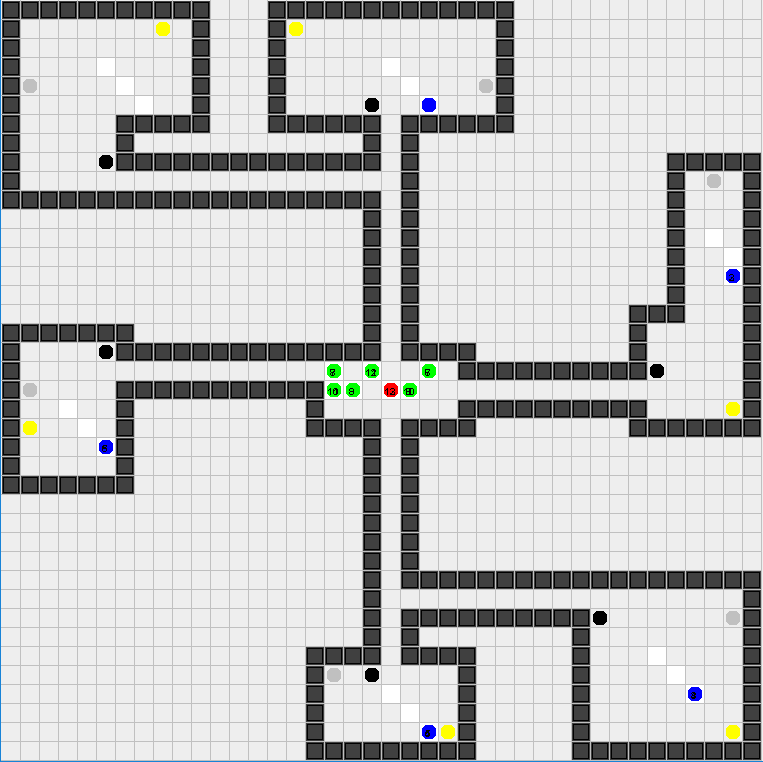
\includegraphics[scale = 0.55]{img/miniera.png}
  \caption{Rappresentazione della miniera}
\end{figure}
Il modello realizzato è formato da una griglia 50x50 che rappresenta una miniera composta da una serie di caverne.\\
Le sezioni nere del modello aiutano a rappresentare (anche visivamente) la sua struttura, delineando ostacoli non attraversabili dagli agenti del sistema.\\
La miniera è logicamente e fisicamente suddivisa dai seguenti elementi:
\begin{itemize}
	\item n.1 \textit{ControlCave}: posizionata al centro dell'intera miniera, è un punto focale di coordinamento per gli agenti.\\
	Ogni \textit{carrier}, infatti, ritornerà periodicamente all'interno di questa cave per ottenere dei compiti da svolgere e/o risorse richieste dai miners (ad esempio, birra).\\Al suo interno risiede staticamente l'unico agente \textit{forger} presente, rappresentato in rosso.\\
	\item n.6 \textit{MineCave}: dimora di ogni \textit{miner} del sistema, è il luogo nel quale le risorse previste del sistema vengono posizionate per essere raccolte.\\ Possono essere di varia forma e, per ipotesi semplificatrice, hanno un unica uscita che porta alla \textit{ControlCave} attraverso una serie di tunnel.\\
	Come già premesso, ogni \textit{MineCave} contiene esclusivamente un \textit{miner} (rappresentato da un pallino di colore blu) e da una serie di punti di interesse, qui elencati:
	\begin{itemize}
		\item Una vena di oro (in giallo)
		\item Una vena di ferro (in grigio)
		\item uno punto di stoccaggio (in nero) delle risorse raccolte localmente
	\end{itemize}\vspace*{0.4cm}
	
	\item \textit{Tunnel}: ogni \textit{MineCave} e collegata alla \textit{ControlCave} attraverso una serie di cunicoli chiamati \textit{Tunnel}.\\ Possono esistere più \textit{Tunnel} consecutivi che conducono a una stessa caverna.\\ Gli unici agenti in grado di percorrerli sono i \textit{carrier}, rappresentati in verde.
\end{itemize}
Ogni tipologia di caverna è una specializzazione della classe astratta \textit{Cave}, ognuna caratterizzata da una lista di oggetti \textit{Area} e un dizionario degli items contenuti: grazie a \textit{jason} e al suo nativo supporto a java, la creazione di un modello del sistema viene così notevolmente semplificata.\\
\begin{figure}
  \centering
   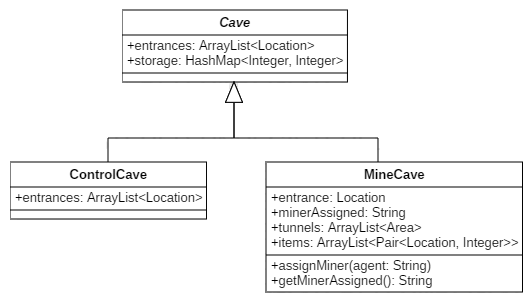
\includegraphics[scale = 0.7]{img/diagramCaves.png}
  \caption{Gerarchia di classi per le caverne della miniera}
\end{figure}
\lstinputlisting[float=h,caption=Cave.java]{code/Cave.java}
\lstinputlisting[float=h,caption=MineCave.java]{code/MineCave.java}
\vspace{21cm}
\lstinputlisting[caption=ControlCave.java]{code/ControlCave.java}
L'ambiente in cui gli agenti sono situati presenta una serie di eventi stocastici che possono cambiare la loro behaviour all'interno della società: ad esempio, ogni dieci secondi esiste il 33\% di probabilità che un orda di orchi minacci la miniera.\\\\
In tal caso, tutti gli agenti reagiranno a tali eventi in base a delle precise direttive: nel suddetto esempio il \textit{forger} inizierà a produrre armature (sempre ammesso che ci siano abbastanza risorse in magazzino), i \textit{miners}scaveranno soltanto ferro e i \textit{carriers} si interesseranno soltanto di prelevarlo dai magazzini locali delle \textit{MineCaves}.
%===========================================================================
%===========================================================================
\newpage
%===========================================================================
\section{Progetto}
\labelsec{Progetto}
Il progetto è stato sviluppato tramite \textit{Jason}, un interprete basato su una versione estesa di AgentSpeak.\\
Come tutti i linguaggi utilizzati per programmare agenti BDI, \textit{Jason} permette di descrivere Belief, Goals e Plans attraverso regole Prolog-Like, oltre a rendere possibile la definizione di piani pienamente compatibili con codice Java.\\
Come già anticipato nell'analisi dei requisiti, sarà opportuno che gli agenti del sistema basino la loro capacità di effettuare scelte intelligenti all'interno del sistema grazie alla combinazione di \textit{Epistemic States} e \textit{Motivational States}.\\\\
Tali caratteristiche sono canonicamente presenti nelle architetture BDI, e possono essere descritte come segue:
\begin{itemize}
	\item Beliefs: rappresentano la conoscenza che un agente ha acquisito dell'ambiente in cui è immerso. In genere, un belief è descritto da un predicato che può essere di valore vero o falso.\\
	\item Desires: rappresentano l'insieme degli obiettivi che un oggetto vorrebbe raggiungere. Un desire si può ritenere soddisfatto quando viene aggiunto al set interno di beliefs oppure quando personalmente scartato.\\
	\item Intentions: rappresentano ciò che l'agente ha deciso di compiere concretamente.
\end{itemize}
\newpage
\subsection{Beliefs}
Ogni agente del sistema possiederà dei personali \textit{Beliefs} che varieranno, ovviamente, per ogni tipologia presente nel sistema(cioè \textit{miner}, \textit{carrier} o \textit{forger}).\\Alcune percezioni verranno aggiunte al proprio insieme di \textit{mental states} solo al seguito di determinati eventi o azioni: la posizione delle vene di materiale all'interno di una miniera, ad esempio, sarà aggiunta ai \textit{mental states} dei miners soltanto una volta completato il proprio plan di "scansione".\\\\
Si tenga conto che la seguente lista di \textit{beliefs} che viene presentata non è da considerarsi esaustiva: verranno infatti presentati soltanto i più significativi a livello didattico.
\subsubsection{Miner Beliefs}~
\lstinputlisting[float=h,caption=Beliefs per l'agente \textit{miner}]{code/beliefs_miner.java}\\
Come facilmente intuibile, il grado di sete del minatore sarà rappresentato dal belief \textit{thirstness(X)}; di conseguenza, il minatore si fermerà ogni operazione di scavo (o di trasporto) quando il belief \textit{thirsty} diverrà true.\\\\
La forza personale del minatore avrà un impatto rilevante sulla quantità di materiale trasportato dal punto di scavo allo storage (rispettivamente rappresentati dai beliefs \textit{strength\textunderscore kg} e \textit{carrying}); a questo scopo, il raggiungimento del limite personale di raccolta verrà indicato dal belief \textit{atCapacity}.\\\\
\textit{direction(Direction)} e \textit{my\textunderscore position} sono dei beliefs utili per la fase di scanning della cave personale del \textit{miner}, in quanto permettono di orientare spazialmente l'agente nell'ambiente.\\\\
\textit{forgerNeeds(Resource)} rappresenta la richiesta corrente di materiale fornita dal \textit{ carrier} per conto del \textit{forger}: al seguito di questa belief addition, il \textit{miner} si adopererà per raggiungere la vena di materiale più vicina e iniziare ad estrarlo.\\\\
Infine, la posizione delle risorse situate nella caverna e del punto di storage sono indicate da \textit{resource(Resource, Location) e storage(Location)}: tali personali credenze verranno aggiunte durante le fasi iniziali di "scansione" della propria caverna.
\subsubsection{Carrier Beliefs}~
\lstinputlisting[float=h,caption=Beliefs per l'agente \textit{carrier}]{code/beliefs_carrier.java}\\
Come per i \textit{miners}, ogni \textit{carrier} possiede dei beliefs in supporto alle operazioni di trasporto, carico e scarico del materiale estratto dalle caverne.\\A livello di codice, le loro modalità di utilizzo si possono considerare sostanzialmente equivalenti a quelle già viste precedentemente sugli agenti scavatori.\\\\
\textit{storageKg} rappresenta la quantità di materiale presente nella cave locale, e sarà azzerato e aggiornato ad ogni raggiungimento di una nuova caverna.\\\\
Con \textit{goCollect(Resource)}, invece, si vuole rappresentare la richiesta corrente di materiale emessa dal forger; al seguito di questa belief addition, il carrier si adopererà per trovare una cave libera per adempiere alla commessa.\\\\
Infine, sono stati aggiunti dei beliefs in supporto agli spostamenti tra caverna e caverna, forniti direttamente (tramite scambio di messaggi) dall'agente \textit{forger} della miniera: un esempio è fornito da \textit{cave(Index,Miner,X,Y)}, che contiene le informazioni sull'indice della caverna, il miner assegnato e la sua posizione spaziale.\newpage
\subsubsection{Forger Beliefs}~
\lstinputlisting[float=h,caption=Beliefs per l'agente \textit{forger}]{code/beliefs_forger.java}\\
L'agente \textit{forger} possiede tutta una serie di beliefs utili per il suo compito di coordinamento della miniera.\\\\
Il bisogno corrente di materiale è esplicitato dal belief \textit{needs(Material)}, che verrà comunicato di volta in volta ad ogni \textit{carrier} (e, di conseguenza, ad ogni \textit{miner} per l'estrazione) una volta raggiunta la \textit{controlCave}.\\Si tenga presente che l'insieme di \textit{carriers} conosciuti dal \textit{forger} è rappresentato da \textit{carrier(Name)}.\\\\La quantità di risorse stoccata nel magazzino principale è rappresentata da \textit{storageKg(Resource, Kg)}, che verrà aggiornato ad ogni consegna degli agenti trasportatori.\\\\
Infine, \textit{orkOrdeIncoming} indica il probabile arrivo di un orda di orchi nella miniera: in tal caso il \textit{forger} comanderà di estrarre solamente FERRO dalle \textit{mineCaves} (cambiando, pertanto, il belief \textit{needs()}) e inizierà a produrre armature per ogni 50kg di materiale.\\
Ogni armatura prodotta verrà indicata da \textit{items(armor, X)}.
\newpage
\subsection{Comportamento}
Il comportamento di ogni agente è definito da una serie di piani che vengono applicati in base alle necessità riscontrate.\\
In questa sezione verranno presentati soltanto i piani più rilevanti di ogni tipologia di agente implementato nel sistema.
\subsubsection{Miner plans}~\\\\
Una volta ricevuto l'ordine di estrazione di materiale, il \textit{miner} eseguirà una serie di operazioni che possono essere riassunte come segue:
\begin{enumerate}
	\item Viene reperito dalla propria \textit{belief base} il più vicino punto di scavo per il materiale richiesto.\\
	Dopodiché, lo si raggiunge fisicamente tramite il plan \textit{goTo(X, Y).}\\
	\item Si procede ad estrarlo tramite il plan \textit{pickup(Resource)}.\\
	\item Si ottiene il posizionamento dello storage locale e lo si raggiunge fisicamente (sempre tramite il plan \textit{goTo(X,Y))}.\\ 
	Una volta raggiunto, si rilascia il materiale trasportato tramite il plan \textit{dropBag}.\\
	\item Infine, il \textit{miner} aggiorna la propria percezione della sete.
\end{enumerate}
\lstinputlisting[float=h,caption=Azione di scavo per l'agente \textit{miner}]{code/comp_miner.java}
\subsubsection{Carrier plans}~\\\\
Come già anticipato, i compiti dei \textit{carriers} non si limitano al semplice trasporto di materiale da caverna a \textit{controlCave}: essi ricoprono infatti un ruolo di vero e proprio supporto per tutte le esigenze riscontrate in miniera.\\\\Un esempio di tali esigenze può essere la richiesta di birra da parte di un \textit{miner}; dato che la produzione all'interno della miniera deve sempre rimanere ai massimi livelli, il soddisfacimento della sete di un lavoratore ricopre sempre la massima priorità rispetto agli altri compiti (mentre è assetato, infatti, un minatore si asterrà dal lavorare).\\\\
Il plan di ottenimento di una birra può essere così riassunto:
\begin{enumerate}
	\item Tramite un operazione di \textit{drop\textunderscore intention()}, viene abbandonata qualsiasi intenzione in corso di svolgimento.\\
	\item Si procede a reperire e raggiungere il punto di partenza della caverna (solitamente posto immediatamente fuori dalla \textit{controlCave)} per poter richiedere una birra al \textit{forger} (tramite un messaggio di tipo \textit{askOne}, cioè sincrono).\\
	\item Dopodiché, si reperisce e raggiunge il punto d'entrata della caverna con il \textit{miner} assetato.\\
	\item E infine si ritorna al lavoro precedentemente lasciato in sospeso.
\end{enumerate}
\lstinputlisting[float=h,caption=Reperimento di birra da parte di un \textit{carrier}]{code/comp_carrier.java}\newpage
\subsubsection{Forger plans}~\\\\
I compiti assegnati all'agente \textit{forger} sono perlopiù di gestione della miniera e dei suoi sottoposti.\\
Un esempio tipico si può riscontrare quando i \textit{carriers} tornano dalla loro operazione di carico/scarico materiale delle caverne di scavo: ogni \textit{carrier} dovrà infatti ricevere prontamente nuove comande da eseguire per massimizzare la produttività.\\\\
Pertanto, ogniqualvolta che un \textit{carrier} ritorna nella \textit{controlCave} (a meno che non sia per ottenere una birra da consegnare ai \textit{miners}) , il \textit{forger} dovrà:
\begin{enumerate}
	\item Aggiornare le sue percezioni sulla quantità totale di materiale stoccato nel magazzino.\\
	\item Interrogarsi su quale sia la risorsa di cui la comunità necessita al momento.\\
	\item E infine comandare al \textit{carrier} appena arrivato di andarne a reperire uno stock.
\end{enumerate}
\lstinputlisting[float=h,caption=Arrivo di un \textit{carrier} dal \textit{forger}]{code/comp_forger.java}\newpage
\section{Conclusioni}
Questo progetto rappresenta un valido caso di studio per la mesa in pratica di alcuni aspetti di autonomia visti durante il corso di Sistemi Autonomi presieduto dal prof. Omicini.\\
Innanzitutto, l'utilizzo di jason come interprete per lo sviluppo del progetto ha consentito di sfruttare appieno la flessibilità e il supporto di un linguaggio comune come Java: la creazione di un modello coerente con gli obiettivi del corso è stata così notevolmente semplificata.\\
In alcuni circoscritti casi sono state definite delle internal actions personalizzate in grado di agire efficacemente sul model dell'applicazione; tuttavia, è necessario sottolineare che la loro implementazione è stata evitata nella maggior parte dei casi grazie a un attento utilizzo di rules e plans minimali.\\
Infine, la decisione di diversificare gli agenti in tre diverse tipologie si è rilevata vincente per riuscire a simulare un MAS di una certa complessità; ciò ha permesso di studiare vari gradi di autonomia e di interazione tra gli agenti del sistema.
\end{document}
